\documentclass[twocolumn, letterpaper]{scrartcl}
\usepackage{padrao_logica}
\newcommand\docID{2018-00}
\newcommand\createdOn{09 de Abril, 2019}

\begin{document}
    \title{\color{triton_blue}LógicaFlow\\ \textit{O que você precisa saber!}}
  %  \author{Lógica Sistemas}
    \date{}

	\maketitle

A popularização das plataformas de comunicação digital acarreta o aumento da quantidade de tráfego de dados. Projeções estimam que até o ano de 2021 o tráfego global de dados móveis será sete vezes maior que aquele em 2016, atingindo 49 exabytes por mês, o que equivale a 49.000.000 gigabytes, em 11,6 bilhões de dispositivos ao redor do mundo. Dado isso, o custo de falhas e problemas de segurança e desempenho se tornam cada vez mais altos, visto que existirão redes mais complexas e uma maior necessidade da garantia da Qualidade de Serviço. Neste contexto, desenvolvemos o LógicaFlow como uma ferramenta baseada no protocolo NetFlow para a análise de fluxo de pacotes com o intuito de encontrar pontos de bloqueio, detectar anomalias na rede, identificar motivos de lentidão, descobrir equipamentos com defeito e analisar comportamento de rede. O objetivo deste documento é mostrar as informações básicas para o entendimento de um sistema de análise de tráfego baseado em NetFlow.%, bem como diferenciar um sistema baseado no protocolo NetFlow dos demais disponíveis no mercado. 

	
\section*{\color{triton_blue}O Aluno de Biologia}

 
Imagine um aluno pesquisador do curso de Biologia que para seu projeto de pesquisa precisa levantar o máximo de informações possíveis sobre um formigueiro, com o objetivo de saber como formigas se comportam como um todo. Ele levanta às 5 da manhã, pega seu lápis, caderno, protetor solar, uma garrafa de água e sai em busca de um formigueiro nas ruas. Quando finalmente encontra um formigueiro de formigas carpinteiras, o aluno começa a anotar o número de formigas que entram e saem do formigueiro (ao menos as que ele consegue contar), o que elas carregam e se estão carregando algo. Após algumas horas de observação, ele começa a perceber que talvez essas informações não sejam suficientes, então começa a seguir as formigas para tentar descobrir alguma nova informação útil. Durante seu percurso, ele percebe que as fileiras de formigas se separam e que cada grupo busca seus recursos em lugares diferentes. No caminho ele também percebe que há uma formiga de serra mais distante, sozinha e carregando um material maior que as demais formigas carpinteiras. Neste momento ele percebe que seu método não é tão eficaz. Além de ter parado de contar quantas formigas entravam ou saiam do formigueiro e o que carregavam para verificar outro comportamento, ele percebeu que tipos diferentes de formigas já não andavam em fileiras, mas sim sozinhas. 

De fato, por mais que ambas sejam formigas, espécies diferentes possuem algumas características de comportamento distintas. Além de não poder generalizar o comportamento das formigas analisando apenas um tipo, o aluno também deixa de obter outras informações ao analisar somente o comportamento de uma única formiga pelo que ela carrega. Se ao invés disso ele analisasse o comportamento da fileira, poderia obter medidas de quantas formigas conseguem sair e voltar do formigueiro por campanha de busca de recursos, qual o recurso mais buscado por campanha, se elas voltam agitadas ou não e até explicar os motivos pelos quais as fileiras encontram problemas no meio ambiente para cumprir suas tarefas, como ataques de outros animais ou pessoas. 



%\textbf{Nesta introdução da seção, comentar brevemente sobre NetFlow, sFlow e SNMP. Tentar trazer uma rápida evolução histórica sobre os três protocolos.}

%\href{http://www.cables-solutions.com/sflow-vs-netflow-vs-snmp-differences.html}{http://www.cables-solutions.com/sflow-vs-netflow-vs-snmp-differences.html}

%\href{https://www.noction.com/blog/netflow-sflow-ipfix-netstream-network-traffic-monitoring-explained}{https://www.noction.com/blog/netflow-sflow-ipfix-netstream-network-traffic-monitoring-explained}

%\href{https://www.plixer.com/blog/netflow/which-netflow-version-v5-v9-flexible-netflow-or-ipfix/}{https://www.plixer.com/blog/netflow/which-netflow-version-v5-v9-flexible-netflow-or-ipfix/}
%Há duas famosas formas de acumular dados de tráfego de fluxo: NetFlow e sFlow. Ambas possuem dois componentes, uma está numa variedade de diferentes dispositivos (BGPs e Switches) e outra está numa gama de diferentes aplicações de monitoramento e análise que processam os dados exportados da primeira parte. 

%\subsection*{\color{triton_blue}sFlow}
%\textbf{Breve explicação do funcionamento sFlow de maneira simples e fácil de entender}
%\subsection*{\color{triton_blue}SNMP}
%\textbf{Breve explicação do funcionamento SNMP de maneira simples e fácil de entender}

\subsection*{\color{triton_blue}Análise de Fluxo}

Uma comparação de maneira análoga pode ser feita com um sistema de análise de fluxo do tráfego de rede. É mais útil analisar um fluxo (fileira) de pacotes (formigas) e poder estimar quais tipos de dados (recursos) trafegam na rede (meio ambiente), qual a taxa máxima de transmissão de dados em diferentes momentos do dia, bem como se todos são transmitidos com sucesso ou se a transmissão está apresentando comportamentos inesperados ou ataques. NetFlow é um protocolo introduzido em roteadores da Cisco (também criado por esta empresa) que considera os pacotes como parte de um fluxo que tem começo, meio e fim ao invés de apenas contá-los, como ocorre em outros protocolos. Hoje, dispositivos encaminhadores de pacotes de outras grandes empresas como MikroTik, Huawei e Juniper também conseguem exportar fluxos de dados. Um fluxo é definido como uma sequência unidirecional de pacotes com algumas propriedades em comum que passam por um dispositivo de rede. Por considerar pacotes como um fluxo, administradores de empresas possuem informações sobre o tráfego de rede de maneira mais abrangente, permitindo um melhor gerenciamento de serviços por meio do monitoramento da rede, planejamento de capacidade, monitoramento e caracterização de aplicações e clientes, análise de segurança, entre outros recursos. 



\begin{figure}[!h]
	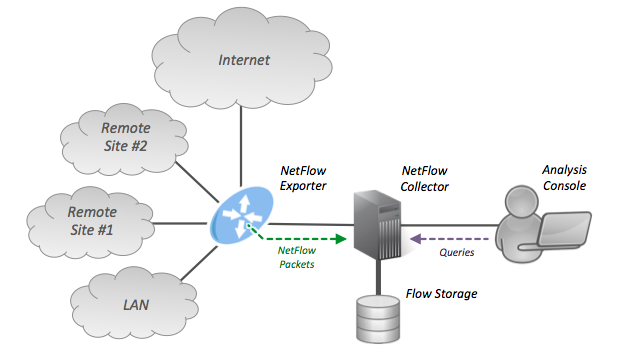
\includegraphics[width=\linewidth]{arquitetura_netflow.png}
	\caption{Arquitetura NetFlow. \label{arqnetflow}}
%		\vspace{0.1in}
%		\includegraphics[width=\linewidth]{example-image-b}
%		\caption{flowchart 2. \label{fig:b}}
\end{figure}	

O Exportador NetFlow, como mostra a Fig.\ref{arqnetflow}, coleta os pacotes no tráfego IP entrando e saindo do dispositivo e os organiza em formato de fluxo com base nos endereços IP de origem e destino em comum, nas portas de origem e destino em comum, no mesmo protocolo da camada de rede, no mesmo tipo de serviço ou na mesma interface lógica. Então, o Exportador NetFlow envia esses fluxos para o Coletor NetFlow, que pode receber fluxos de um ou mais exportadores. O papel do Coletor NetFlow é processar os fluxos recebidos, ou seja, organizar e armazenar esses dados. O LógicaFlow funciona como o agente analisador dos fluxos armazenados. Em posse desses dados, somos capazes de mostrar a quantidade de tráfego por portas, detectar ataques tipo Distributed Denial of Service (DDoS), as taxas de Download e Upload por serviço, entre outros. A quantidade de informações possíveis a serem extraídas dos fluxos é enorme e podem ser moldadas de acordo com as necessidades do cliente! Se houvesse um LógicaFlow para formigas, os problemas do estudante estariam resolvidos!

%The NetFlow Collector receives Flow Records from one or more Exporters.  It processes the received Export Packet(s); that is, it parses and stores the Flow Record information.  Flow Records can be optionally aggregated before being stored on the hard disk.  The NetFlow Collector is also referred to as the Collector in this document.





    %\section*{\color{triton_blue}Second Section}

	
    
   % \subsection*{\color{triton_blue}Subsection}

% https://en.wikibooks.org/wiki/LaTeX/Bibliography_Management#Embedded_system
    \bibliographystyle{unsrtnat}
    %\bibliography{biblio}
    
%    \begin{thebibliography}{9}
    
 %   \end{thebibliography}
    
	\blurb
\end{document}
